\subsection{The CLAS12 Forward Detector}
\label{fd}
\vspace{0.3cm}\noindent
The FD consist of of a Torus magnet, a large 6-coil superconducting magnet symmetrically arranged surrounding the beam line.
The Torus magnet is sandwiched between a drift chamber tracking system with a total of 36 layers arranged in 3 regions (R1, R, R3)
of 12 layers each. in each of the six Torus sectors R1  located at the entrance to the magnet, R2 inside the magnet and R3 just after the magnet, providing independent and redundant tracking in each of the six Torus sectors. Each of the 3 regions consists of 6 layers with
wires strung at $\Delta{\phi} = 84^\circ$ from sector mid plane and 6 layers with wires strung at $\Delta{\phi} = 96^\circ$ from
sector mid plane.  This "stereo" view enables good resolution in the azimuthal scattering angle. Cherenkov counters, time-of-flight detectors
and calorimeters are located  downstream of the tracking system to provide identification and energy measurements for
electrons, high energy photons, and neutrons.  In this section we describe each of these systems, but refer for full details to the
individual detector articles.




\subsection{High Threshold Cherenkov Counter (HTCC)}
\label{htcc}
\vspace{2cm}
\begin{figure}[h]
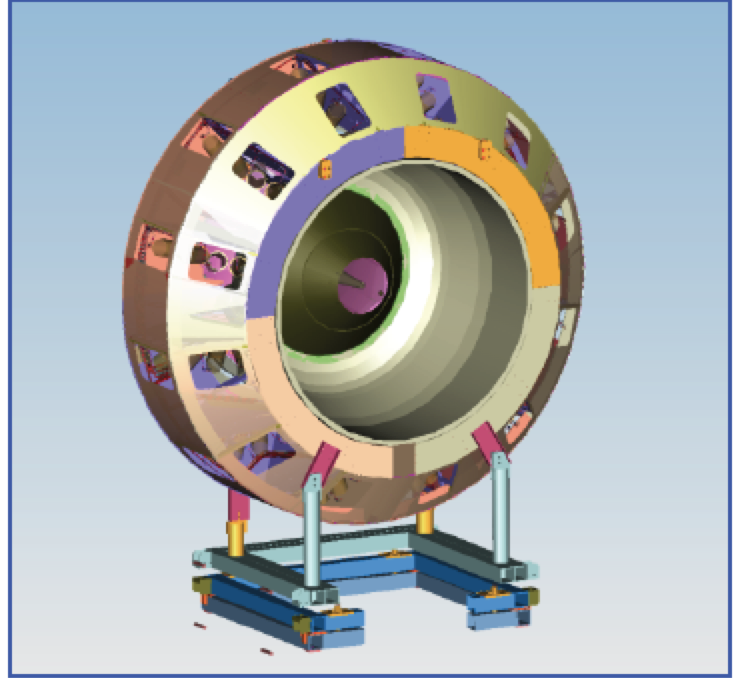
\includegraphics[width=0.5\columnwidth]{HTCC-pic.png}
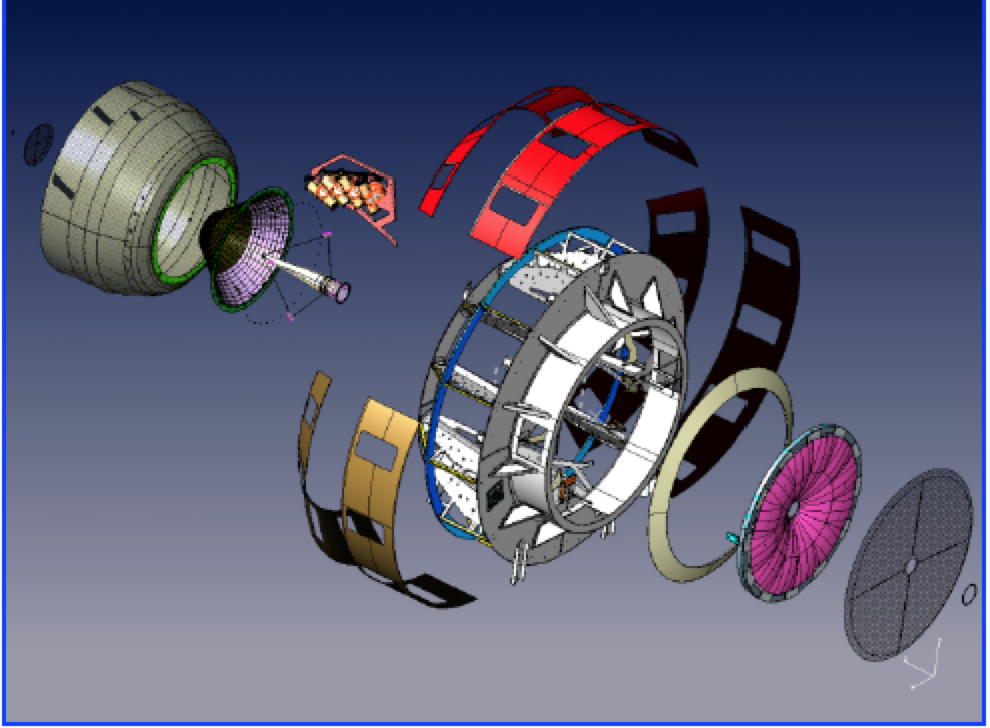
\includegraphics[width=0.5\columnwidth]{HTCC-components-pic.png}
\caption{Left: The assembled HTCC system. Right: The components of the HTCC in exploded view.
The HTCC is used to generate a fast trigger signal to be used as a trigger for scattered electrons.
It is located in front of the Torus magnet and the drift chamber tracking detectors. It presents a minimal amount of
inactive material to limit its impact on the tracking performance. It consists of 60 lightweight composite ellipsoidal
mirrors. Its active volume extends over the full azimuthal angle.  }
\end{figure}
\subsection{Central Time-of-Flight Detector (CTOF)}
Function, design features, performance, 1 figure
\begin{figure}[]
\hspace{3.0cm}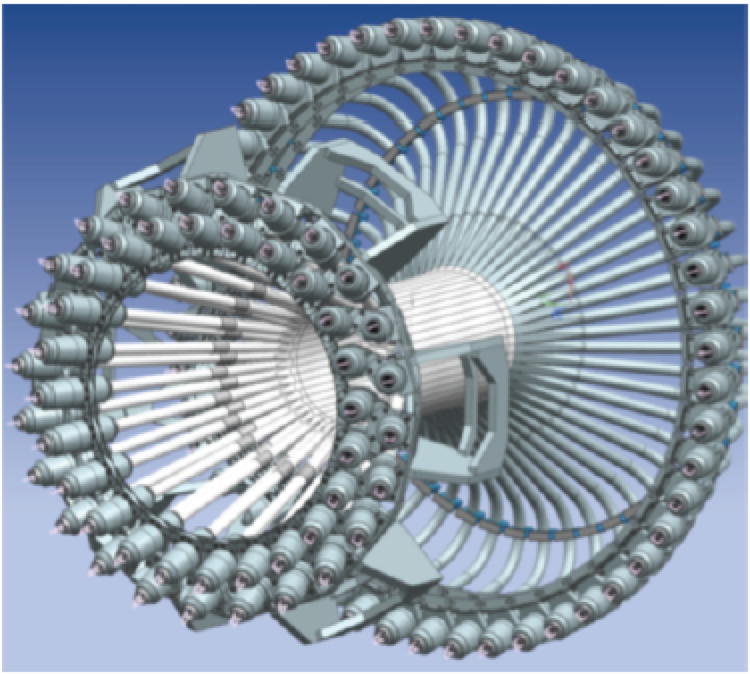
\includegraphics[width=0.5\columnwidth]{CTOF-pic.png}
\caption{The Central Time-=of-Flight system is used for the identification of charged particle emerging
from the target via time-of-flight measurements. The CTOF includes 48 plastic scintillators with
double-sided photomultiplier readout via 1 m long
upstream and 1.6m-long downstream focusing light guides.}
\end{figure}
%\vfill\eject

\subsubsection{Forward MicroMesh Gas Detectors}
General description, function, performance

\subsubsection{Low Threshold Cherenkov Counters (LTCC)}
\label{ltcc}
1 Figure for performance
\vspace{0.3cm}\noindent
\subsubsection{Ring Imaging Cherenkov Counter (RICH)}
\label{rich}
1 Figure construction, 1 figure performance
\vspace{0.3cm}\noindent
\subsubsection{Forward Time-of-Flight Counters (FTOF)}
\label{ftof}
1 Figure construvtion, 1 figure performance
\vspace{0.3cm}\noindent
\subsubsection{Electromagnetic Calorimeters (PCAL/ECAL }
\vspace{0.3cm}\noindent
1 Figure construction (PCAL), 1 figure performance PCAL+EC
